\subsection{Handling the imbalance (E3)}

Fig.~\ref{fig:imbalance} crosses three training strategies with two
threshold rules. Three findings stand out.

\emph{Re-balancing does not make the strong models rank better.} For Random
Forest and XGBoost, class weights and SMOTE change PR-AUC by about one point at
most (XGBoost: \ImbXGBNonePRAUC{} without, \ImbXGBSmotePRAUC{} with SMOTE). For
Logistic Regression and the MLP they make it slightly worse.

\emph{Re-balancing mostly moves the decision boundary.} At the fixed 0.5
threshold, class weights and SMOTE push Logistic Regression towards
high recall and very low precision (F1 \ImbLRNoneFixedFone{} $\rightarrow$
\ImbLRWeightFixedFone{}). The same shift is available, more cleanly, by choosing
the threshold.

\emph{Threshold tuning helps weak models but not the trees.} A tuned threshold
lifts Logistic Regression from \ImbLRNoneFixedFone{} to \ImbLRNoneTunedFone{}
and the MLP from \ImbMLPNoneFixedFone{} to \ImbMLPNoneTunedFone{}. For the Random
Forest, the threshold tuned on validation steps is \emph{worse} than 0.5
(\ImbRFNoneTunedFone{} vs \ImbRFNoneFixedFone{}). The best threshold moves over
time: it is a property of the period, not of the model. We still report tuned
thresholds as the main result, because 0.5 being better is only visible in
hindsight.

\begin{figure}[t]
  \centering
  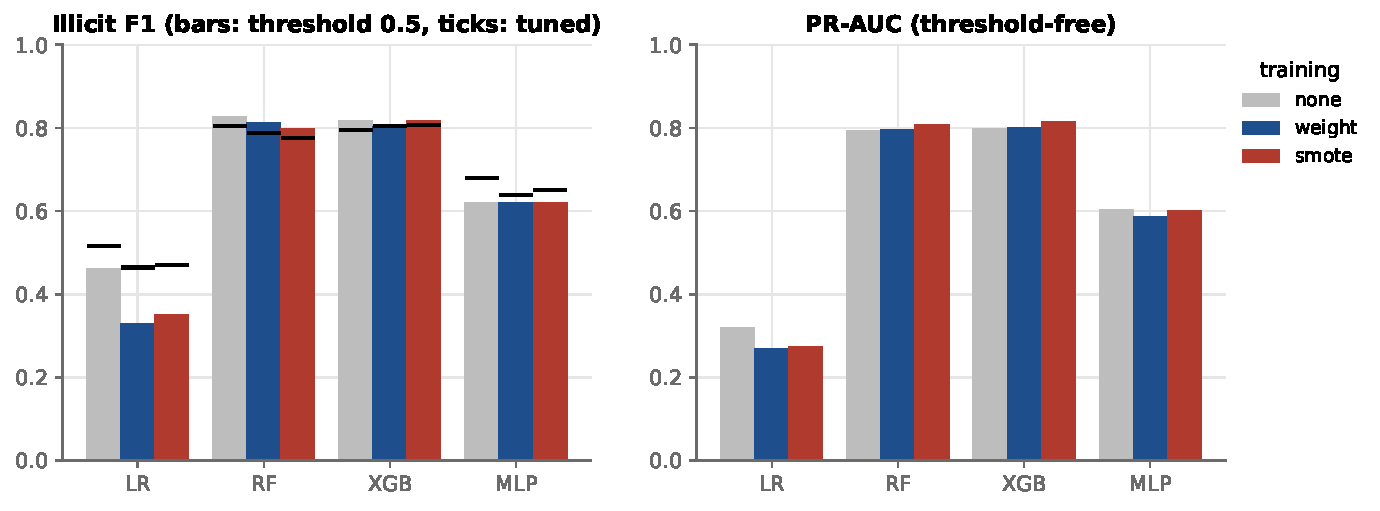
\includegraphics[width=\columnwidth]{../reports/figures/e03_imbalance.pdf}
  \caption{Imbalance strategies. Left: illicit F1 at threshold 0.5 (bars) and at
  the validation-tuned threshold (ticks). Right: PR-AUC. Mean of five seeds.}
  \label{fig:imbalance}
\end{figure}
